\documentclass[10pt,aspectratio=169,mathserif]{beamer}
\usepackage{nju}
\usepackage[UTF8]{ctex}
\usepackage{xeCJK}
\usepackage{amsmath,amsfonts,amssymb,bm}
\usepackage{color}
\usepackage{ulem}
\usepackage{graphicx,hyperref,url}
\usepackage{listings}
% \usepackage{minted}

\lstset{
    language=C++, % 设置语言为C++
    backgroundcolor=\color{white}, % 设置背景色为黑色
    basicstyle=\ttfamily\color{black}\footnotesize, % 设置字体为Consolas,并设置为白色
    keywordstyle=\color{blue}, % 设置关键字的颜色
    commentstyle=\color{green!60!black}, % 设置注释的颜色
    stringstyle=\color{purple}, % 设置字符串的颜色
    numbers=left, % 显示行号
    numberstyle=\tiny\color{gray}, % 设置行号的样式和颜色
    frame=single, % 设置代码框的边框样式
    breaklines=true, % 自动换行
    tabsize=4, % 设置制表符的宽度
      columns=fullflexible, % 处理制表符
}


\beamertemplateballitem
% \catcode`\。=\active                  %或者=13
% \newcommand{。}{.}    
%将正文中的“。”号转换为“.”。

\title{C++ 高级程序设计-经验分享}

\author[熊丘桓]{
    熊丘桓\ 软件学院\\
  {\small \url{eaglebear@smail.nju.edu.cn}}}

\date{\today}

\begin{document}

\begin{frame}
    \titlepage
\end{frame}

\begin{frame}
    \frametitle{目录}
    \tableofcontents
\end{frame}

\section{分享目的}
\begin{frame}{\sout{免责声明}分享目的}
    \begin{itemize}
        \item 咨询任课老师和助教以获取考试内容和考试题型。
        \item 分享个人学习经验和工程经验,供参考之用。
    \end{itemize}
\end{frame}

\section{设计理念}
\begin{frame}{设计理念}
    \begin{enumerate}
        \def\labelenumi{\arabic{enumi}.}
        \item
              效率
        \item
              实用性优于艺术性严谨性
        \item
              允许一个有用的特征比防止各种错误使用更重要(相信程序员)
    \end{enumerate}
\end{frame}

\section{设计的结果}
\begin{frame}{设计的结果}
    \begin{itemize}
        \item
              相比于 Java 并不优美的 OO 语法
        \item
              相比于 C 增加了更反直觉且难以理解的执行逻辑
        \item
              开发端最紧缺的岗位之一:C++ 工程师
    \end{itemize}

    但如果你理解了 C++ 的理念和目的,那么以上问题都能迎刃而解

\end{frame}

\section{三条主要脉络}
\begin{frame}
    \begin{center}
        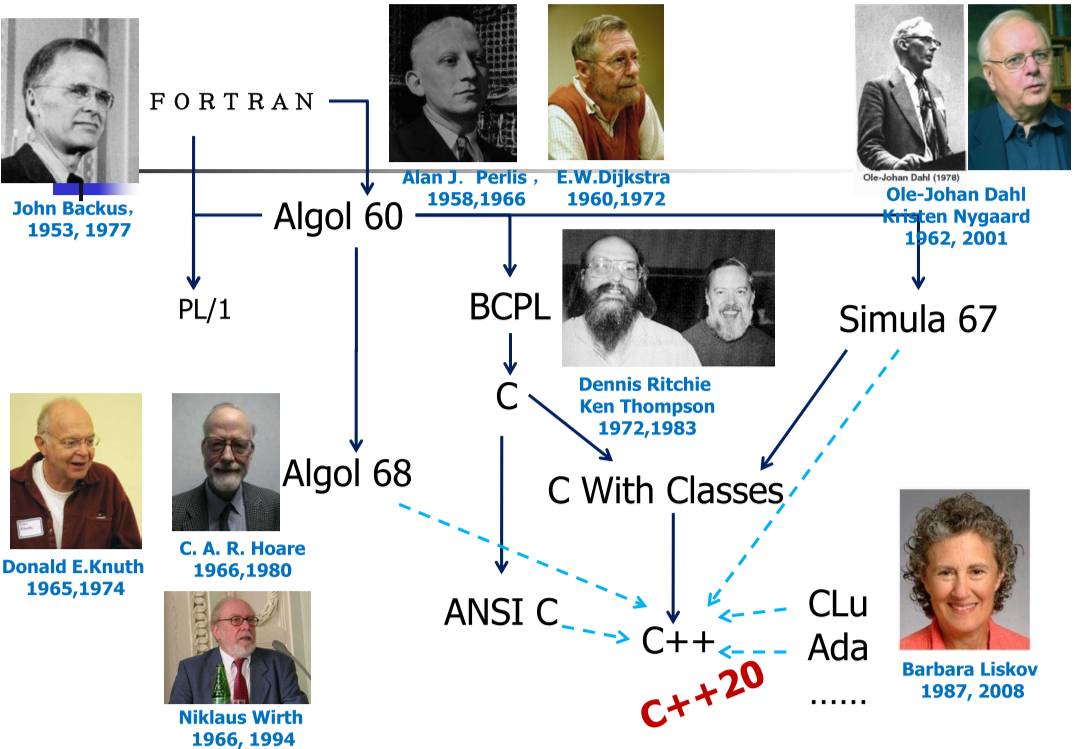
\includegraphics[height=\textheight]{image/c++_history.png}
    \end{center}
\end{frame}

\begin{frame}{三条主要脉络}
    \begin{itemize}
        \item
              Algo60:结构化编程,拒绝意大利面条!
        \item
              BCPL \& C:系统编程,程序员可以摸到 CPU 和内存
        \item
              Simula67:OO 编程,梦开始的地方
    \end{itemize}
\end{frame}



\section{不同人眼里的 C++}

\begin{frame}{不同人眼里的 C++}

    \begin{itemize}
        \item
              算法竞赛选手:C++ = C + STL
        \item
              Java 选手:C++ = C + OO
        \item
              面经魔怔人:C++ = \&\ldots{}*\$\#@
        \item
              软院选手:C++ = 比 CPL 更简单的机试题,面向往年卷复习
        \item
              苏州校区选手:往年卷?什么往年卷?
    \end{itemize}

\end{frame}


\section{归纳的考试重点}
\begin{frame}{\sout{我猜的}根据软院往年卷归纳的考试重点}

    \begin{enumerate}
        \def\labelenumi{\arabic{enumi}.}
        \item
              多态:重载(overload)与重写(override)
        \item
              函数的运行机制:传值和传引用

              \begin{quote}
                  C 语言:你猜我为什么不支持重载?
              \end{quote}
        \item
              宏:上古时期的\sout{奇技淫巧}魔法
        \item
              常量指针和指针常量:CPL 笔试的漏网之鱼
        \item
              C++ 为什么比 Java 难:五三原则、虚函数、多继承
        \item
              \href{https://eaglebear2002.github.io/2022Spring-C++\%20\%E9\%AB\%98\%E7\%BA\%A7\%E7\%A8\%8B\%E5\%BA\%8F\%E8\%AE\%BE\%E8\%AE\%A1/C++\%20\%E9\%AB\%98\%E7\%BA\%A7\%E7\%A8\%8B\%E5\%BA\%8F\%E8\%AE\%BE\%E8\%AE\%A1-25-\%E9\%9D\%A2\%E5\%90\%91\%E5\%AF\%B9\%E8\%B1\%A1\%E7\%BC\%96\%E7\%A8\%8B\%E5\%8D\%81\%E5\%A4\%A7\%E9\%97\%AE\%E9\%A2\%98/}{面向对象编程十大问题}
    \end{enumerate}
\end{frame}

\section{例题}
\begin{frame}
    \vfill
    \centering
    \Large 恭喜你!你已经精通 C++ 啦\\
    下面来做几道例题吧
    \vfill
\end{frame}

\begin{frame}[fragile]
    \begin{lstlisting}
// 例题 1:函数重载
void bar(int i) { cout << "bar(1)" << endl; }
void bar(const char c) { cout << "bar(2)" << endl; }
void func(int a) { cout << "func(1)" << endl; }
void func(char c) { cout << "func(2)" << endl; }
void func(long long ll) { cout << "func(3)" << endl; }
void hum(int i, ...) { cout << "hum(1)" << endl; }
void hum(int i, int j) { cout << "hum(2)" << endl; }
int main() {
    char c = 'A';
    bar(c);
    short s = 1;
    func(s);
    hum(12, 5);
    hum(10, 12, 1);
    system("pause");
}
\end{lstlisting}
\end{frame}

\begin{frame}[fragile]
    \begin{lstlisting}
// 例题 1:函数重载
void bar(int i) { cout << "bar(1)" << endl; }
void bar(const char c) { cout << "bar(2)" << endl; }
void func(int a) { cout << "func(1)" << endl; }
void func(char c) { cout << "func(2)" << endl; }
void func(long long ll) { cout << "func(3)" << endl; }
void hum(int i, ...) { cout << "hum(1)" << endl; }
void hum(int i, int j) { cout << "hum(2)" << endl; }
int main() {
    char c = 'A';
    bar(c); // bar(2)
    short s = 1;
    func(s); // func(1)
    hum(12, 5); // hum(2)
    hum(10, 12, 1); // hum(1)
    system("pause");
}
\end{lstlisting}
\end{frame}

\begin{frame}[fragile]
    \begin{lstlisting}
// 例题 2:常量和指针
int main() {
const int c = 128;
    int* q = const_cast<int*>(&c); // 强制类型转换
    *q = 111; // 企图通过变量指针修改常量
    cout << " c " << &c << c << endl;
    cout << " q " << &q << q << endl;
    cout << "*q " << q << *q << endl;
}
\end{lstlisting}
\end{frame}

\begin{frame}[fragile]
    \begin{lstlisting}
// 例题 2:常量和指针
int main() {
    const int c = 128;
    int* q = const_cast<int*>(&c); // 强制类型转换
    *q = 111; // 企图通过变量指针修改常量
    cout << " c " << &c << c << endl;
    // c 是符号常量,在编译时符号常量已经变为 128,相当于 define
    // 被编译器当作:cout << " c " << &c << 128 << endl;
    cout << " q " << &q << q << endl;
    cout << "*q " << q << *q << endl;
    //Name   Addr     Value
    // c    0012FF74    128
    // q    0012FF70    0012FF74
    //*q    0012FF74    111
    //对于同一个地址 0x0012FF74,输出了不同的值
}
\end{lstlisting}
\end{frame}

\begin{frame}[fragile]
    \begin{lstlisting}
// 例题 3:右值引用
class A {
    int val;
    void setVal(int v) {
        val = v;
    }
};

A getA() {
    return A();
}

// 知道风险,并且想要改变新对象,就使用右值引用 &&
int main() {
    int a = 1;
    int &ra = a;
    const A &cra = getA();
    A &&aa = getA();
    A &ab = getA();
}
    \end{lstlisting}
\end{frame}

\begin{frame}[fragile]
    \begin{lstlisting}
// 例题 3:右值引用
class A {
    int val;
    void setVal(int v) {
        val = v;
    }
};

A getA() {
    return A();
}

// 知道风险,并且想要改变新对象,就使用右值引用 &&
int main() {
    int a = 1;
    int &ra = a; // OK,非 const 引用绑定左值
    const A &cra = getA(); // OK,const 引用绑定右值
    A &&aa = getA(); // OK,右值引用绑定右值
    A &ab = getA(); // ERROR,引用不能绑定右值
}
    \end{lstlisting}
\end{frame}

\begin{frame}[fragile]
    \begin{lstlisting}
// 例题 4:const 的含义
const void show(const A* const this) const {
    // const 分别是什么含义?
}
    \end{lstlisting}
\end{frame}

\begin{frame}[fragile]
    \begin{lstlisting}
// 例题 4:const 的含义
const void show(const A* const this) const {
    // 第一个 const 修饰指针,表示 this 指针不可修改;
    // 第二个 const 修饰 this,表示 this 指向的对象不可修改;
    // 函数签名当中的 const 相当于参数当中第二个 const
    // 返回值当中的 const:自己去试一试呢?
}
    \end{lstlisting}
\end{frame}

\begin{frame}[fragile]
    \begin{lstlisting}
// 例题 5:构造函数
class Computer {
private:
    const string name;
    Keyboard& keyboard;

public:
    Computer() {
        // 想一想,这么写有什么问题?
        name = "EagleBear2002's PC";
        keyboard = new Keyboard();
    }
}
    \end{lstlisting}
\end{frame}

\begin{frame}[fragile]
    \begin{lstlisting}
// 例题 5:构造函数
class Computer {
private:
    const string name;
    Keyboard& keyboard;

public:
    Computer(): name("EagleBear2002's PC"), key(new Keyboard()) {
        // 成员初始化表:你猜我是干嘛的?
    }
}
    \end{lstlisting}
\end{frame}

\section{}
\begin{frame}[fragile]
    \vfill
    \centering
    \Large 新年快乐,期末大吉!\\
    \sout{让我看看是谁元旦还要复习考试啊}
    \vfill
\end{frame}

\end{document}

